\subsection{Previous Simulations of Atomic Force Microscopy Images}

Currently, there are a limited number of AFM imaging simulations, leaving a prominent area for development. Recent work by Amyot R, Flechsig H  \textit{et al.}. \cite{amyot2020bioafmviewer} produced the BiomolecularAFMviewer in 2020. The BiomolecularAFMviewer, similar to this project, uses protein structural data to simulate AFM images (shown in Figure \ref{fig: BioAFMviewer}) and aids in interpreting experimental observations. In follow-up work in 2022, Amyot R, Flechsig H  \textit{et al.}.\cite{amyot2022simulation} used the software to reconstruct resolution-limited experimental images as an example of the application of the software. The modelling used a hard sphere model of the surface and indenter, evaluating the vertical height of the tip at the initial surface-surface contact. Therefore, the simulation does not account for indentation into the surface, surface deflection, off-axial forces that produce sliding and friction, or elastic properties of the surface. This approach could be improved by accounting for force curves and the indentation of the tip with elastic properties of the material. 

\begin{figure}[H]
    \centering
    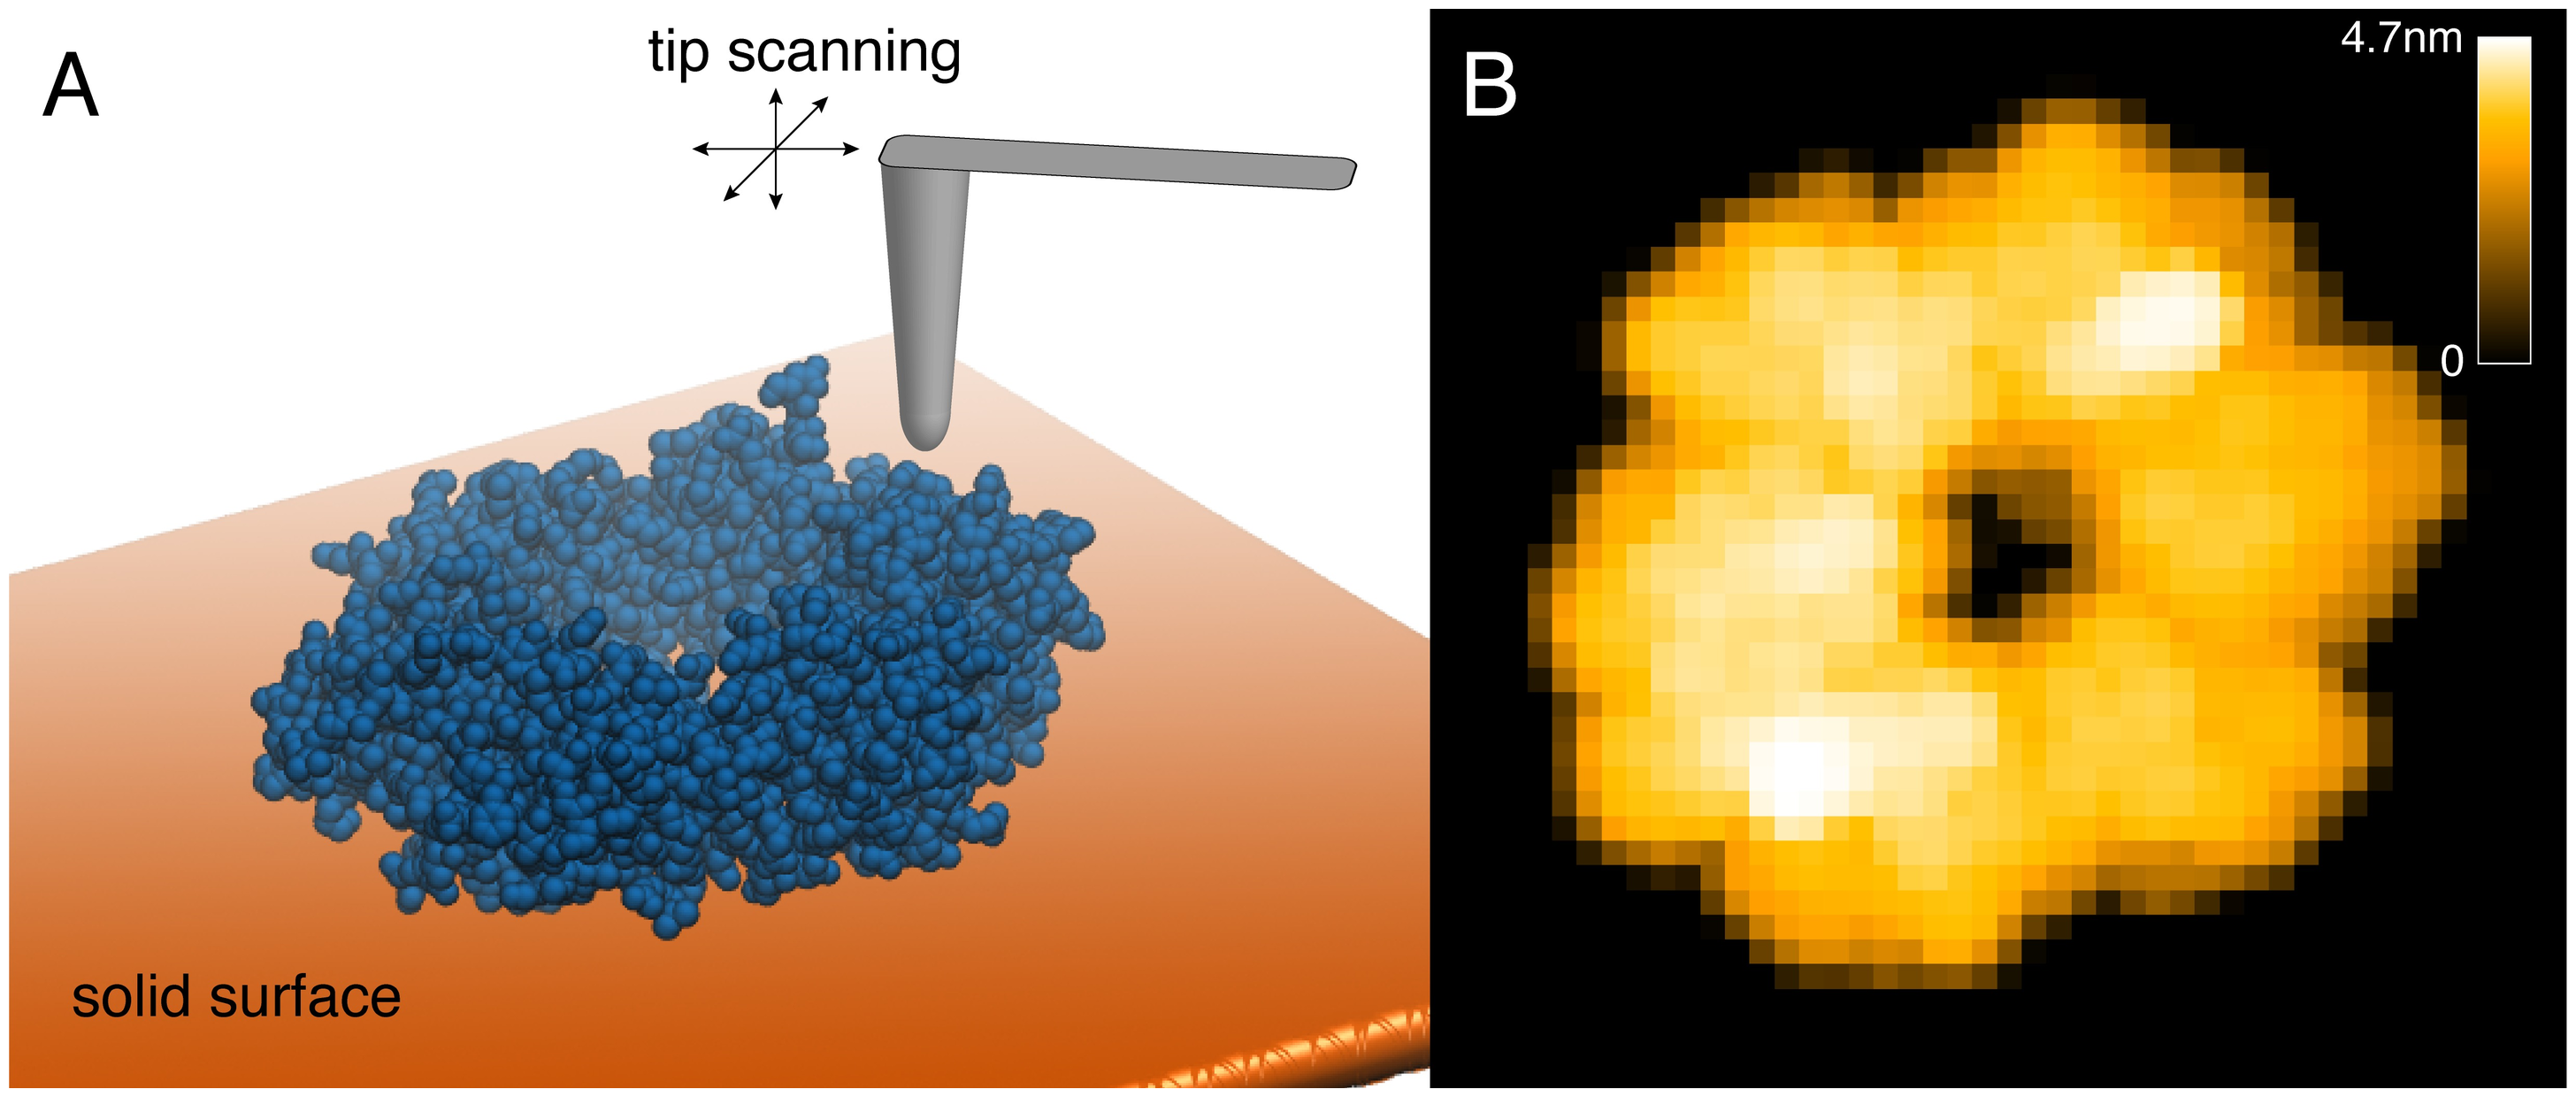
\includegraphics[width=0.8\linewidth]{Figures/BioAFMviewer.png}
    \caption{Graphic of simulation from BioAFMviewer\cite{amyot2020bioafmviewer}. (A) 3D geometry of simulation. (B) Simulated AFM image.}
    \label{fig: BioAFMviewer}
\end{figure}

Other computational simulations of AFM have been used to produce such force curves that reflect these properties. However, these applications study quantitative AFM results as opposed to imaging \cite{liu2019finite,han2021modified,kontomaris2020hertz,senda2016computational}. Previous work has shown the viability of the commercial software ABAQUS and Finite Element Modelling (FEM) in the study of indention in AFM; Liu \textit{et al.}\cite{liu2019finite} validated a FEM model for AFM indention with less than 10\% error when comparing the simulated force-indentation curves with the experimental data. Similar analysis of experimental data with FEM done by Roduit \textit{et al.}\cite{roduit2009stiffness} and Han \textit{et al.}\cite{han2021modified} made use of the ABAQUS software to complete calculations. The work by Rajabifar \textit{et al.}.\cite{rajabifar2021fast} simulated the viscoelasticity contact between an AFM tip and a surface. This showed a fast and accurate use of FEM to simulate AFM indentation and the associated force curves. 